
\centering
\rule{0}{12.5cm}
:(

\begin{minipage}[t][][]{0.47\linewidth}
\raggedright
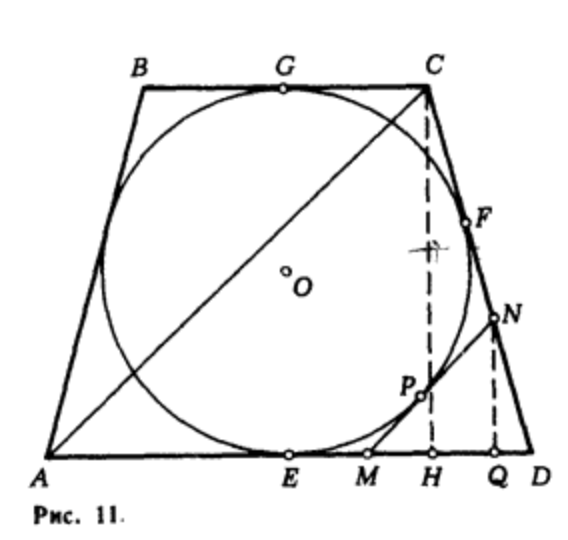
\includegraphics[scale=0.75]{1.png}
треугольник LHE также будет равнобедренным. Поэтому
$ |OM|=\sqrt{|OL|^2-|LM|^2}=\sqrt{(|LH|-|OH|)^2-|ME|^2}=\sqrt{(|LE|-|OH|)^2-|KF|^2}=\sqrt{(\frac{8}{3}b-b)^2-(\frac{4}{3}b)^2}=b $\\
Используя подобие треугольников ACD и LOM с коэффициентом подобия $ k = \frac{|AC|}{|LO|}=\frac{2|AO|}{|LH|-|OH|}=\frac{2(|AL|+|LH|-|OH|)}{|LE|-|OH|}=\frac{2(\frac{8}{3}b+\frac{8}{3}b-b)}{\frac{8}{3}b-b}=5,2 $, находим искомую площадь $S_{ABCD}=2S_{\triangle ACD}=2k^2S_{\triangle LOM}=k^2*|LM|*|OM|=(5,2)^2*\frac{4}{3}b*b=(36\frac{4}{75})b^2$
\vskip6pt
\hspace{2em}Задача 9 (МФТИ, 1974). Около окружности описана равнобедренная трапеция с основаниями AD и BC (|AD|>|BC|). Прямая, параллельная диагонали AC, пересекает стороны AD и CD соответственно в точках M и N и касается окружности в точке P. Определить углы трапеции, если \(\frac{|MP|}{|PN|}=k\). \\
\vskip6pt
\hspace{2em}Рассмотрение подобных треугольников ACD и MND (рис. 11) приводит к несложному геометрическому решению. Обозначим через E, F и G точки касания окружности со сторонами AD, CD
\end{minipage}
\begin{minipage}[t][][]{0.5\linewidth}
и BC соответственно, через H и Q – проекции точек C и N на сторону AD. Положим ${|PN|=1}$. Тогда $|MP|=k$, $|AH|=|AE|+|EH|=|ED|+|GC|=|DF|+|FC|=|DC|$. Из свойств подобия и в треугольнике MND будет $|MQ|=|DN|$. Поэтому \vskip6pt$|MN|=|MP|+|PN|=k+1$, $|DQ|=|DE|-|QM|-|ME|=|DF|-|DN|-|MP|=|NF|-|MP|=|NP|-|MP|=1-k$, $2|NQ|^2=(|MQ|^2+|NQ|^2)-(|DN|^2-|NQ|^2)=|MN|^2-|DQ|^2=(k+1)^2-(1-k)^2=4k$,$|NQ|=\sqrt{2k}$.
\vskip6ptСледовательно, $tg\widehat{D}=\frac{|NQ|}{|DQ|}=\frac{\sqrt{2k}}{l-k}$, $\widehat{A}=\widehat{D}=arctg\frac{\sqrt{2k}}{l-k}$, $\widehat{B}=\widehat{C}=\pi-arctg\frac{\sqrt{2k}}{l-k}$.
\vskip6pt
\hspace{2em}\textit{Упражнения}
\vskip6pt
\hspace{2em}\textbf{1. }(МГУ, филологич. ф-т. отделение структурной и прикладной лингвистики. 1978). Пятиугольник ABCDE вписан в окружность единичного радиуса. Известно, что $|AB|=\sqrt{2}$, $\widehat{ABE}=45\degree$,$\widehat{EBD}=30\degree$ и $|BC|=|CD|$. Чему равна площадь пятиугольника? \\
\textbf{2. }(МГУ, геологич. ф-т. 1978). В треугольнике ABC длина стороны AB равна 4. $\widehat{CAB}=\frac{\pi}{3}$, а радиус описанной окружности R равен 2,2. Доказать, что длина высоты, опущенной из вершины C на сторону AB, строго меньше $\frac{11\sqrt{3}}{5}$. \\
\textbf{3. }(НГУ, 1976). В паралеллограмме ABCD угол BAD равен $60\degree$. Окружность, проходящая через точки A, B и D, пересекает сторону CD в середине. Найти площадь паралеллограмма, если радиус окружности равен R \\
\textbf{4. }(МГУ, ф-т. почвоведения, 1977). Основание AB трапеции ABCD вдвое длиннее основания CD и вдвое длиннее боковой стороны AD. Длина диагонали AC равно a, а длина боковой стороны BC равна b. Найти площадь трапеции. \\
\end{minipage}
\newpage
\begin{center}
   \centeringКВАНТ. 1998/№6 
\end{center}
\textbf{Элементы планетных орбит}\\
\resizebox{\textwidth}{!}{

\renewcommand{\arraystretch}{2} 
\begin{tabular}{ |c|c|c|c|c|c|c|c|c|c| } 
\hline
Планета & \multicolumn{2}{|c|}{\makecell{Среднее \\расстояние\\ от солнца}} & \multicolumn{2}{|c|}{\makecell{Сидерический \\период \\обращения}} & \multirow{2}{*}{\rotatebox{90}{\parbox{3.75cm}{\makecell[l]{Синодерический \\период, в \\средних сутках}}}} & \makecell{Эксцентри-\\ситет ($\epsilon$)} & \makecell{Наклон \\орбиты (i)} & \multicolumn{2}{|c|}{\makecell{Расстояние от Земли, \\ в млн км}}\\
\cline{2-3} \cline{4-5} \cline{9-10}

& в а.е & \makecell{в млн\\ км} &\makecell{ в тропич. \\годах }& \makecell{ в средн. \\сутках} & \rule{0pt}{4em}& & & наименьшее & наибольшее \\
\hline
Меркурий & 0,387 & 57,9 & 0,241 & 87,97 & 115,88 & 0,206 & $7\degree00'$ & 82 & 217 \\
Венера   & 0,723 & 108,2  & 0,615 & 224,70 & 583,92 & 0,007 & 3 24 & 39  & 260  \\
Земля    & 1,000 & 149,6  & 1,000 & 365,26 & - & 0,017 & 0 00 & --  & --   \\ 
Марс     & 1,524 & 227,9  & 1,880 & 686,98 & 779,94& 0,093 & 1 51 & 56  & 400  \\ 
Юпитер   & 5,203 & 778,3  & 11,862 & 4332,59 & 398,88 & 0,048 & 1 18 & 591 & 965  \\ 
Сатурн   & 9,539 & 1433,5 & 29,458 & 10759,20& 378,09 & 0,054 & 2 29 & 1199& 1653 \\ 
Уран     & 19,191& 2871,0 & 84,015 & 30685,93& 369,66 & 0,046 & 0 46 & 2586& 3153 \\ 
Нептун   & 30,071& 4498,6 & 164,788& 60187,64& 367,48 & 0,008 & 1 46 & 4309& 4682 \\ 
Плутон   & 39,529& 5913,5 & 247,697& 90471,85&366,72 & 0,253 & 17 08 & 4249& 7558 \\ \hline
\end{tabular}
}